\documentclass{article}
\usepackage[utf8]{inputenc}
\usepackage[margin=1.0in]{geometry}
\usepackage{amsmath}
\usepackage{amssymb}
\usepackage{fancyhdr}
\usepackage{physics}
\usepackage{wrapfig}
\usepackage{hyperref}
\usepackage{multirow}
\usepackage{amsthm}
\usepackage{pgfplots}

\pgfplotsset{compat=1.16}



\renewcommand{\thesubsection}{\thesection\Alph{subsection}}
\renewcommand\qedsymbol{\square}



\title{Quantum Mechanics PS3}
\author{Joe Crowley}
\date{October 2020}

\pagestyle{fancy}
\renewcommand{\headrulewidth}{0pt}
\renewcommand{\footrulewidth}{1pt}

\fancyhf{}
\rhead{
Joe Crowley \\
Physics 215 \\
Problem Set 2\\
}
\rfoot{Page \thepage}

\begin{document}  

\section{}
\textit{Suppose a $2 \times 2$ matrix $X$ (not necessarily Hermitian or unitary) is written as
$$
X=a_{0}+\sigma \cdot \mathrm{a}
$$
where $a_{0}$ and $a_{1,2,3}$ are numbers.}
\subsection{}
\textit{How are $a_{0}$ and $a_{k}(k=1,2,3)$ related to $\mathbf{tr}(X)$ and $\mathbf{tr}\left(\sigma_{k} X\right) ?$}
\subsection{}
\textit{Obtain $a_{0}$ and $a_{k}$ in terms of the matrix elements $X_{i j}$}

\newpage

\section{}
\textit{Using the orthonormality of $|+\rangle$ and $|-\rangle,$ prove
$$
\left[S_{i}, S_{j}\right]=i \varepsilon_{i j k} \hbar S_{k}, \quad\left\{S_{i}, S_{j}\right\}=\left(\frac{\hbar^{2}}{2}\right) \delta_{i j}
$$
where
$$
\begin{array}{l}
S_{x}=\frac{\hbar}{2}(|+\rangle\langle-|+|-\rangle\langle+|), \quad S_{y}=\frac{i \hbar}{2}(-|+\rangle\langle-|+|-\rangle\langle+|) \\
S_{z}=\frac{\hbar}{2}(|+\rangle\langle+|-|-\rangle\langle-|)
\end{array}
$$}


\newpage

\section{}
\textit{Construct $|\mathbf{S} \cdot \hat{\mathbf{n}} ;+\rangle$ such that
$$
\mathbf{S} \cdot \hat{\mathbf{n}}|\mathbf{S} \cdot \hat{\mathbf{n}} ;+\rangle=\left(\frac{\hbar}{2}\right)|\mathbf{S} \cdot \hat{\mathbf{n}} ;+\rangle
$$
where $\hat{\mathbf{n}}$ is characterized by the angles shown in the accompanying figure. Express your answer as a linear combination of $|+\rangle$ and $|-\rangle .[$Note: The answer is
$$
\cos \left(\frac{\beta}{2}\right)|+\rangle+\sin \left(\frac{\beta}{2}\right) e^{i \alpha}|-\rangle
$$
But do not just verify that this answer satisfies the above eigenvalue equation. Rather, treat the problem as a straightforward eigenvalue problem. Also, do not use rotation operators, which we will introduce later in this book.$]$}


\newpage
\section{}
\textit{The Hamiltonian operator for a two-state system is given by
$$
H=a(|1\rangle\langle 1|-| 2\rangle\langle 2|+| 1\rangle\langle 2|+| 2\rangle\langle 1|)
$$
where $a$ is a number with the dimension of energy. Find the energy eigenvalues and the corresponding energy eigenkets $($as linear combinations of $|1\rangle and |2\rangle$ $)$.}

\newpage

\section{}
\textit{A two-state system is characterized by the Hamiltonian
$$
H=H_{11}|1\rangle\left\langle 1\left|+H_{22}\right| 2\right\rangle\langle 2|+H_{12}[|1\rangle\langle 2|+| 2\rangle\langle 1|]
$$
where $H_{11}, H_{22},$ and $H_{12}$ are real numbers with the dimension of energy, and |1\rangle and |2\rangle are eigenkets of some observable $(\neq H) .$ Find the energy eigenkets and the corresponding energy eigenvalues. Make sure that your answer makes good sense for $H_{12}=0 .$ (You need not solve this problem from scratch. The following fact may be used without proof:
$$
(\mathbf{S} \cdot \hat{\mathbf{n}})|\hat{\mathbf{n}} ;+\rangle=\frac{\hbar}{2}|\hat{\mathbf{n}} ;+\rangle
$$
with $|\hat{n} ;+\rangle$ given by
$$
|\hat{\mathbf{n}} ;+\rangle=\cos \frac{\beta}{2}|+\rangle+e^{i \alpha} \sin \frac{\beta}{2}|-\rangle
$$
where $\beta$ and $\alpha$ are the polar and azimuthal angles, respectively, that characterize $\hat{\mathbf{n}}$. }

\begin{figure}[h!]
    \centering
    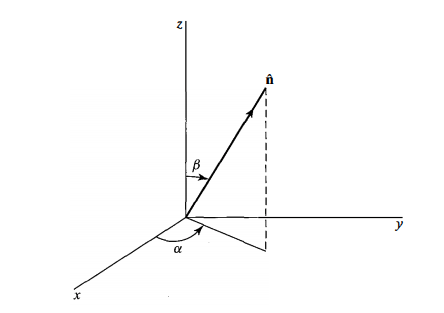
\includegraphics{figures/problem5.png}
    \label{fig:my_label}
\end{figure}

\end{document}
